\subsection{Named entry recognition}

Named-entity recognition (NER) refers to a data extraction. It's a task that is responsible for finding, storing and sorting textual content into default categories such as the names of persons, locations, organizations, quantities, expressions of times, monetary values and percentages. That's what we have to do.

\subsubsection{Glove}

GloVe is an unsupervised learning algorithm for obtaining vector representations for words. Training is performed on aggregated global word-word co-occurrence statistics from a corpus, and the resulting representations showcase interesting linear substructures of the word vector space.

The Euclidean distance (or cosine similarity) between two word vectors provides an effective method for measuring the linguistic or semantic similarity of the corresponding words. Sometimes, the nearest neighbors according to this metric reveal rare but relevant words that lie outside an average human's vocabulary.

Pre-trained word vectors. This data is made available under the Public Domain Dedication and License v1.0 whose full text can be found at: \\http://www.opendatacommons.org/licenses/pddl/1.0/.
\begin{itemize}
    \item Wikipedia 2014 + Gigaword 5 (6B tokens, 400K vocab, uncased, 50d, 100d, 200d, \& 300d vectors, 822 MB download): glove.6B.zip
    \item Common Crawl (42B tokens, 1.9M vocab, uncased, 300d vectors, 1.75 GB download): glove.42B.300d.zip
    \item Common Crawl (840B tokens, 2.2M vocab, cased, 300d vectors, 2.03 GB download): glove.840B.300d.zip
    \item Twitter (2B tweets, 27B tokens, 1.2M vocab, uncased, 25d, 50d, 100d, \& 200d vectors, 1.42 GB download): glove.twitter.27B.zip
\end{itemize}

For the sake of ease, the writing below is used to obtain these data:

\begin{lstlisting}
    wget -P ./data/ "http://nlp.stanford.edu/data/glove.6B.zip"
    unzip ./data/glove.6B.zip -d data/glove.6B/
    rm ./data/glove.6B.zip
\end{lstlisting}


\subsubsection{Prepare data}

For the data, the coNLL database was used. It contains training data, test data during training, and test data after training. These data are in the form of:

\begin{lstlisting}
    CRICKET O
    - O
    LEICESTERSHIRE I-ORG
    TAKE O
    OVER O
    AT O
    TOP O
    AFTER O
    INNINGS O
    VICTORY O
    . O
    
    LONDON I-LOC
    1996-08-30 O
    
    West I-MISC
    Indian I-MISC
    all-rounder O
    Phil I-PER
    Simmons I-PER
    took O
    ...
\end{lstlisting}

where first word is the label and second one is the tag. The space between words represents the end of a sentence and the beginning of another.

These data must be processed before they get to "feed" the neural network. So for that we need a list of distinct word sets, a list of tags and a list of characters. These lists are required to correctly distribute the number of neurons on each layout in the neural network.

To read the data, an iterable class was used that reads a sentence and returns the list of words and character list. These lists may contain duplicates.

\begin{lstlisting}[language=Python,caption={Read data}]
    def __next_sentence(self):
        words, tags = [], []
        while True:

            try:
                line = next(self.file_stream)
            except Exception as e:
                if len(words) != 0:
                    return words, tags

                self.rest_stream()
                raise e

            line = line.strip()

            if len(line) == 0 or line.startswith("-DOCSTART-"):
                if len(words) != 0:
                    return words, tags
            else:
                line_words = line.split(' ')

                words += [self.processing_word(line_words[0]) if self.processing_word is not None else line_words[0]]
                tags += [self.processing_tag(line_words[1]) if self.processing_tag is not None else line_words[1]]
\end{lstlisting}

But we need that lists do not contain duplicates. For this python is the best ally, there is a date type called "set" that does this for you:\\

\begin{lstlisting}[language=Python,caption={Make vocabular}]
    def make_vocab(self):
        vocab_words = set()
        vocab_tags = set()
        vocab_chars = set()
        for words, tags in self:
            vocab_words.update(words)
            vocab_tags.update(tags)

        for word in vocab_words:
            vocab_chars.update(word)

        self.rest_stream()

        return vocab_words, vocab_tags, vocab_chars
        
\end{lstlisting}

\subsubsection{Build graph}

TensorFlow can be regarded as a great promise structure. This means that the graph must first be built. So let's start by declare some placeholders that will represent the graph entries.

\begin{lstlisting}[language=Python,caption={Add placeholders}]
    # shape = (batch size, max length of sentence in batch)
    self.word_ids = tf.placeholder(tf.int32, [None, None], "word_ids")
    
    # shape = (batch size)
    self.sequence_lengths = tf.placeholder(tf.int32, [None], "sequence_lengths")
    
    # shape = (batch size, max length of sentence in batch, max length of word in sentence)
    self.char_ids = tf.placeholder(tf.int32, [None, None, None], "char_ids")
    
    # shape = (batch_size, max_length of sentence in batch)
    self.word_lengths = tf.placeholder(tf.int32, [None, None], "word_lengths")
    
    # shape = (batch size, max length of sentence in batch)
    self.labels = tf.placeholder(tf.int32, [None, None], "labels")
    
    # randomize variables (layouts)
    self.dropout = tf.placeholder(tf.float32, [], "dropout")
    
    # learn rate
    self.lr = tf.placeholder(tf.float32, [], "lr")
        
\end{lstlisting}

All placeholders have the first dimension "bach\_size" because we want to train a certain number on the statements at the same time. This is good for imposing network performance.

Now define the first node in the graph, namely the words. The "embedding\_lookup" function will look for "word\_ids" ids in the parameter list. That is, it will collect the representation of the words trained by the network. Embedding words (represented by words as vector) will be provided by Glove.

\begin{lstlisting}[language=Python,caption={Add word embeddings}]
    with tf.variable_scope("words"):
        self._word_embeddings = tf.Variable(
            self.config.embeddings,
            dtype=tf.float32,
            trainable= False,
            name="_word_embeddings")

        # shape (?, ?, self.config.dim_word)
        self.word_embeddings = tf.nn.embedding_lookup(self._word_embeddings, self.word_ids, name="word_embeddings")

        # for tensorboard
        tf.summary.histogram('_word_embeddings', self._word_embeddings)
        
\end{lstlisting}

For the sake of greater accuracy, the same thing was done for the characters of the words. But this time the network will train this layout itself.

\begin{lstlisting}[language=Python,caption={Add char embeddings}]
    with tf.variable_scope("chars"):
        # get char embeddings matrix
        _char_embeddings = tf.get_variable(
            dtype=tf.float32,
            shape=[self.config.n_chars, self.config.dim_char],
            name="_char_embeddings")

        # shape (?, ?, ?, self.config.dim_char)
        char_embeddings = tf.nn.embedding_lookup(_char_embeddings, self.char_ids, name="char_embeddings")

        # for tensorboard
        tf.summary.histogram('_char_embeddings', _char_embeddings)
        
\end{lstlisting}

Until now we have the layouts defined, so we have to apply "lstm" on them. To meet the "bidirectional\_dynamic\_rnn" conditions, you must reshapes "char\_embeddings" and "word\_lengths".

\begin{lstlisting}[language=Python,caption={Apply bi-LSTM to char embeddings}]
    # make it to fit
    # because word lengths depends by bach_size; sentence can have different lengths
    s = tf.shape(char_embeddings)
    bach_size = s[0]
    max_length_sentence= s[1]
    mas_length_word = s[2]
    char_embeddings = tf.reshape(char_embeddings, [bach_size * max_length_sentence, mas_length_word, self.config.dim_char], "char_embeddings")
    word_lengths = tf.reshape(self.word_lengths, [bach_size * max_length_sentence], "word_lengths")

    cell_fw = tf.contrib.rnn.LSTMCell(self.config.hidden_size_char, state_is_tuple=True)
    cell_bw = tf.contrib.rnn.LSTMCell(self.config.hidden_size_char, state_is_tuple=True)
    _, ((_, output_fw), (_, output_bw)) = tf.nn.bidirectional_dynamic_rnn(cell_fw, cell_bw, char_embeddings, sequence_length=word_lengths, dtype=tf.float32)

    # read and concat output
    output = tf.concat([output_fw, output_bw], axis=-1)

    # shape = (batch size, max sentence length, char hidden size)
    output = tf.reshape(output, [bach_size, max_length_sentence, 2 * self.config.hidden_size_char], "output")
        
\end{lstlisting}

Now we just need to add this piece to the graph and attach the placeholder to randomization. This is very easy by using tensorflow.

\begin{lstlisting}[language=Python,caption={Randomize the word embeddings}]
    word_embeddings = tf.concat([self.word_embeddings, output], axis=-1)
    self.word_embeddings = tf.nn.dropout(word_embeddings, self.dropout)   
\end{lstlisting}

Most to do the same thing for word embeddings. This will help to capture context of words.

\begin{lstlisting}[language=Python,caption={Apply bi-LSTM to word embeddings}]
    cell_fw = tf.contrib.rnn.LSTMCell(self.config.hidden_size_lstm)
    cell_bw = tf.contrib.rnn.LSTMCell(self.config.hidden_size_lstm)
    (output_fw, output_bw), _ = tf.nn.bidirectional_dynamic_rnn(cell_fw, cell_bw, self.word_embeddings, sequence_length=self.sequence_lengths, dtype=tf.float32)
    
    output = tf.concat([output_fw, output_bw], axis=-1)
    output = tf.nn.dropout(output, self.dropout)
        
\end{lstlisting}

Now you have to add the last layout, which predicts what kind of tag will be assigned to the word "interrogated". For this we will let tensorflow calculate the required number of nodes in the tensor.

\begin{lstlisting}[language=Python,caption={Add last layout}]
    W = tf.get_variable("W", dtype=tf.float32, shape=[2 * self.config.hidden_size_char_lstm, self.config.n_tags])

    b = tf.get_variable("b", shape=[self.config.n_tags], dtype=tf.float32, initializer=tf.zeros_initializer())

    s = tf.shape(output)
    output = tf.reshape(output, [-1, 2 * self.config.hidden_size_char_lstm])
    pred = tf.matmul(output, W) + b
    self.logits = tf.reshape(pred, [-1, s[1], self.config.n_tags])

    # for tensorboard
    tf.summary.histogram('W', W)
        
\end{lstlisting}

For the actual prediction, CRF was used. Also, the formula error with which the "reduce\_mean" error is calculated is added. And also for good performances was added AdamOptimizer. 

\begin{lstlisting}[language=Python,caption={Add loss and optimizer}]
    # -log(x)
    log_likelihood, trans_params = tf.contrib.crf.crf_log_likelihood(self.logits, self.labels, self.sequence_lengths)
    
    self.trans_params = trans_params  # need to evaluate it for decoding
    self.loss = tf.reduce_mean(-log_likelihood)
    
    # for tensorboard
    tf.summary.scalar("loss", self.loss)
    tf.summary.histogram("histogram loss", self.loss)
    
    tf.train.AdamOptimizer(self.lr).minimize(self.loss)
\end{lstlisting}


The final graph will look like in \figurename {\ref{fig:finalGraph}}. In this figure is show all nodes in the graph. The image was automatically made by TensorBoard based on the previously built graph.

\begin{figure}[H]
  \centering
  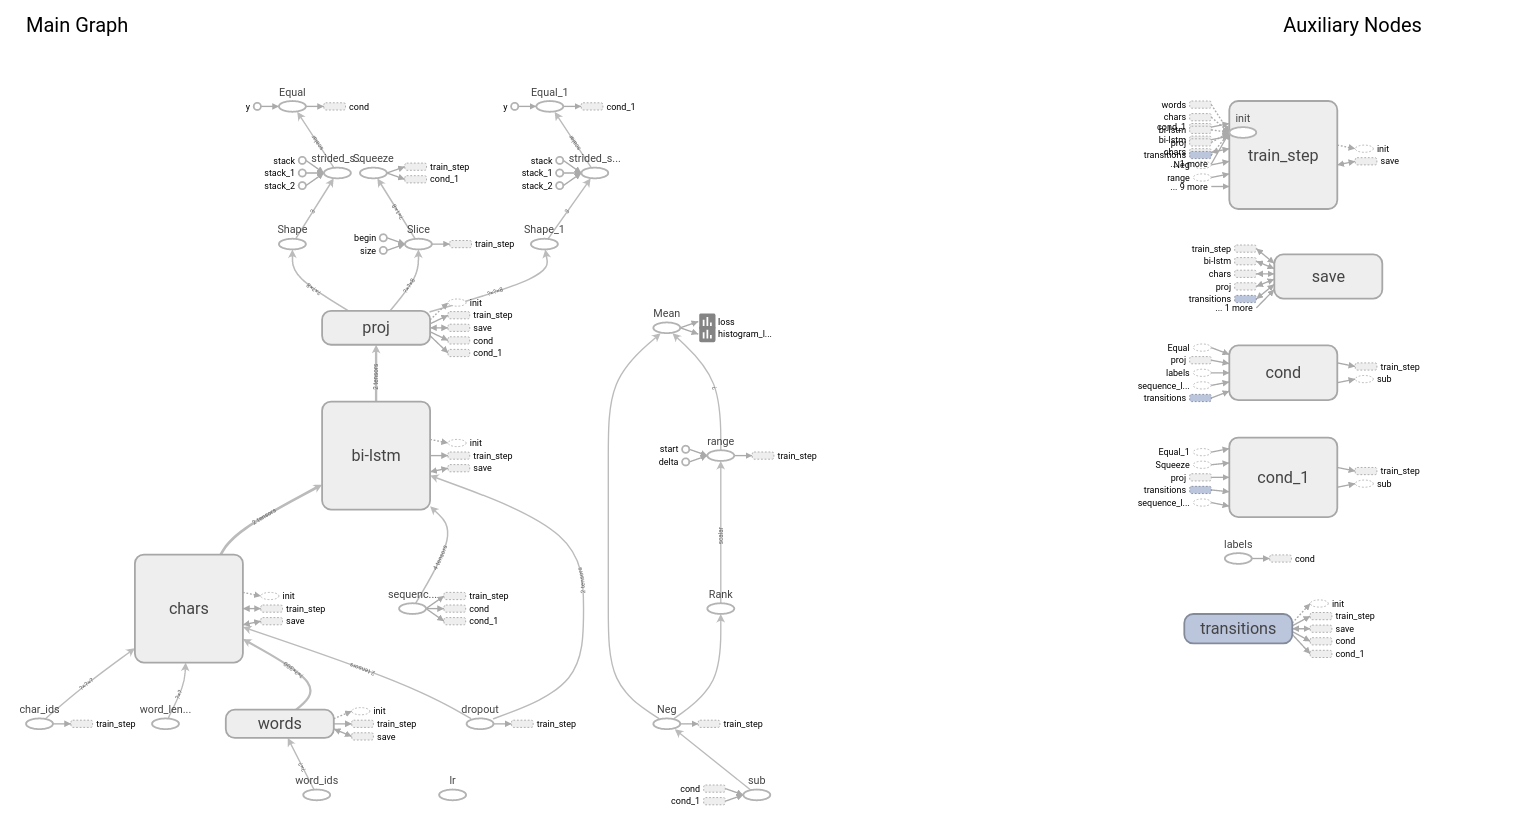
\includegraphics[width=6.5in]{images/finalGraph.png}
  \caption {Final graph}
  \label{fig:finalGraph}
\end{figure}

We now have the built-in network, now it has to be trained and tested.

\begin{lstlisting}[language=Python,caption={Train network}]
    def train(self, train: CoNLLDataset, dev: CoNLLDataset):
        best_score = 0
        n_epoch_no_improve = 0  # for early stopping
    
        for epoch in range(self.config.n_epochs):
            score = self._run_epoch(train, dev, epoch)
            self.config.lr *= self.config.lr_decay  # decay learning rate
    
            if score >= best_score:
                n_epoch_no_improve = 0
                best_score = score
                self.save_session()
            else:
                n_epoch_no_improve += 1
                if n_epoch_no_improve >= self.config.n_epoch_no_improve:
                    break
    
    def _run_epoch(self, train: CoNLLDataset, dev: CoNLLDataset, epoch) -> int:
        n_batches = (len(train) + self.config.batch_size - 1) // self.config.batch_size

        # iterate over dataset
        for i, (words, labels) in enumerate(minibatches(train, self.config.batch_size)):
            fd, _ = self.get_feed_dict(words, labels, self.config.lr, self.config.dropout)

            _, train_loss, summary = self.sess.run([self.train_op, self.loss, self.merged], feed_dict=fd)

        metrics = self._run_evaluate(dev)

        return metrics["f1"]
\end{lstlisting}

As mentioned above, the network will be fed with a small number of sentences of the same length. So for that we need a tool that uniformises sentences and characteristics too. In other words, to transforms the words in there ids based on the dictionary and bring them in the same form.

\begin{lstlisting}[language=Python,caption={Make embeddings}]
    def pad_sequences(sequences, sequences_length=None):
        sequences_length = max(
            map(lambda x: len(x) if type(x) is not int else 0, sequences)) if sequences_length is None else sequences_length
    
        seqs = []
        lengths = []
        for sequence in sequences:
    
            seq = fill_array(sequence if type(sequence) is not int else [sequence], sequences_length)
            length = len(sequence) if type(sequence) is not int else 0
    
            if type(sequence) is not int and type(sequence[0]) == list:
                max_length_word = max([max(map(lambda x: len(x), _seq)) for _seq in sequences])
    
                # seq = list(map(lambda x: [x] if type(x) == int else x, seq))
                seq, length = pad_sequences(seq, max_length_word)
    
            lengths += [length]
            seqs += [seq]
    
        return seqs, lengths
\end{lstlisting}

Now we can feed the network. For that need to fit placeholders dimensions.

\begin{itemize}
    \item word\_ids: (batch size, max length of sentence in batch)
    \item sequence\_lengths: (batch size)
    \item char\_ids: (batch size, max length of sentence in batch, max length of word in sentence)
    \item word\_lengths: (batch size, max length of sentence in batch)
    \item labels: (batch size, max length of sentence in batch)
\end{itemize}

\begin{lstlisting}[language=Python,caption={Feed network}]
    def get_feed_dict(self, words, labels=None, lr=None, dropout=None):

        char_ids, word_ids = zip(*words)

        word_ids, sequence_lengths = pad_sequences(word_ids)
        char_ids, word_lengths = pad_sequences(char_ids)

        # build feed dictionary
        feed = {
            self.word_ids: word_ids,
            self.sequence_lengths: sequence_lengths,
            self.char_ids: char_ids,
            self.word_lengths: word_lengths
        }

        if labels is not None:
            labels, _ = pad_sequences(labels)
            feed[self.labels] = labels

        if lr is not None:
            feed[self.lr] = lr

        if dropout is not None:
            feed[self.dropout] = dropout

        return feed, sequence_lengths
\end{lstlisting}

There are two types of evaluation for neural network, one based on exact match (f1) and index matching.

In statistical analysis of binary classification, the F1 score (also F-score or F-measure) is a measure of a test's accuracy. It considers both the precision p and the recall r of the test to compute the score: p is the number of correct positive results divided by the number of all positive results returned by the classifier, and r is the number of correct positive results divided by the number of all relevant samples (all samples that should have been identified as positive). The F1 score is the harmonic average of the precision and recall, where an F1 score reaches its best value at 1 (perfect precision and recall) and worst at 0.

\begin{equation*}
     F_1=2 * \frac {precision * recall} {precision + recall}
\end{equation*}

\begin{lstlisting}[language=Python,caption={Test network}]
    def _run_evaluate(self, test: CoNLLDataset):
        accs = []
        correct_preds, total_correct, total_preds = 0., 0., 0.
        for words, labels in minibatches(test, self.config.batch_size):
            labels_pred, sequence_lengths = self.predict_batch(words)

            for lab, lab_pred, length in zip(labels, labels_pred,
                                             sequence_lengths):
                lab      = lab[:length]
                lab_pred = lab_pred[:length]
                accs    += [a==b for (a, b) in zip(lab, lab_pred)]

                cond = lambda x: x[0] != self.config.vocab_tags[NONE]   

                lab_chunks = set(filter(cond, get_chunks(lab, self.config.vocab_tags)))
                lab_pred_chunks = set(filter(cond, get_chunks(lab_pred, self.config.vocab_tags)))

                correct_preds += len(lab_chunks & lab_pred_chunks)
                total_preds += len(lab_pred_chunks)
                total_correct += len(lab_chunks)

        p = correct_preds / total_preds if correct_preds > 0 else 0
        r = correct_preds / total_correct if correct_preds > 0 else 0
        f1 = 2 * p * r / (p + r) if correct_preds > 0 else 0
        acc = np.mean(accs)

        return {"acc": 100 * acc, "f1": 100 * f1}

    def predict_batch(self, words):

        fd, sequence_lengths = self.get_feed_dict(words, dropout=1.0)

        viterbi_sequences = []
        logits, trans_params = self.sess.run([self.logits, self.trans_params], feed_dict=fd)

        for logit, sequence_length in zip(logits, sequence_lengths):
            logit = logit[:sequence_length] 
            viterbi_seq, viterbi_score = tf.contrib.crf.viterbi_decode(logit, trans_params)
            viterbi_sequences += [viterbi_seq]

        return viterbi_sequences, sequence_lengths
\end{lstlisting}

\subsubsection{Tests}

Reteteau has been tested on several types of configurations. The best results were obtained with the following configurations.

\begin{lstlisting}[language=Python,caption={Network configurations}]
    n_epochs = 5
    dropout = 0.5  # rate to randomize
    batch_size = 20  # nb of sentence
    lr_method = "adam"
    lr = 0.001  # learn rate
    lr_decay = 0.9  # adjust learn rete
    n_epoch_no_improve = 3

    hidden_size_char_lstm = 100  # lstm on chars
    hidden_size_word_lstm = 300  # lstm on word embeddings
\end{lstlisting}

It is to be noted that the training of the network takes about 25 minutes with these configurations.

\begin{lstlisting}[language=Python,caption={Network results during training}]
    2018-04-15 00:31:01,504 - logger - INFO - Initializing tf session
    2018-04-15 00:31:02,658 - logger - INFO - Epoch 1 out of 5
    2018-04-15 00:36:10,565 - logger - INFO - acc 97.13 - f1 81.56
    2018-04-15 00:36:10,990 - logger - INFO - - new best score!
    2018-04-15 00:36:10,990 - logger - INFO - Epoch 2 out of 5
    2018-04-15 00:41:07,991 - logger - INFO - acc 97.67 - f1 86.18
    2018-04-15 00:41:08,586 - logger - INFO - - new best score!
    2018-04-15 00:41:08,586 - logger - INFO - Epoch 3 out of 5
    2018-04-15 00:46:02,616 - logger - INFO - acc 97.97 - f1 88.25
    2018-04-15 00:46:03,339 - logger - INFO - - new best score!
    2018-04-15 00:46:03,339 - logger - INFO - Epoch 4 out of 5
    2018-04-15 00:50:58,869 - logger - INFO - acc 98.18 - f1 89.35
    2018-04-15 00:50:59,477 - logger - INFO - - new best score!
    2018-04-15 00:50:59,477 - logger - INFO - Epoch 5 out of 5
    2018-04-15 00:55:53,944 - logger - INFO - acc 98.22 - f1 89.87
    2018-04-15 00:55:54,455 - logger - INFO - - new best score!
\end{lstlisting}

One of the results obtained after training is the following
\begin{equation*}
    acc = 97.21;
    f1 = 85.23;
\end{equation*}


\begin{figure}[H]
  \centering
  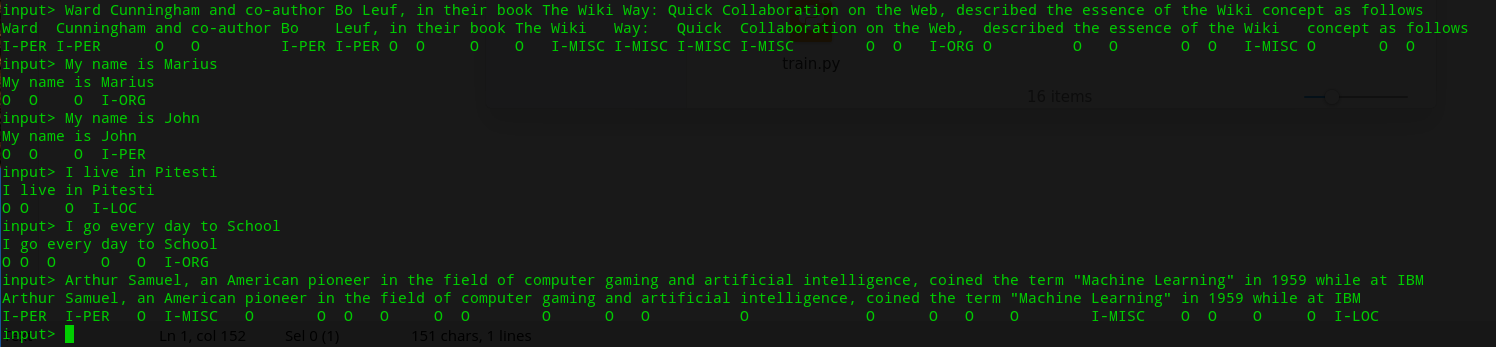
\includegraphics[width=6.5in]{images/interactive.png}
  \caption {Some of the interactive results}
\end{figure}

Here's how the loss diagram shows:

\begin{figure}[H]
  \centering
  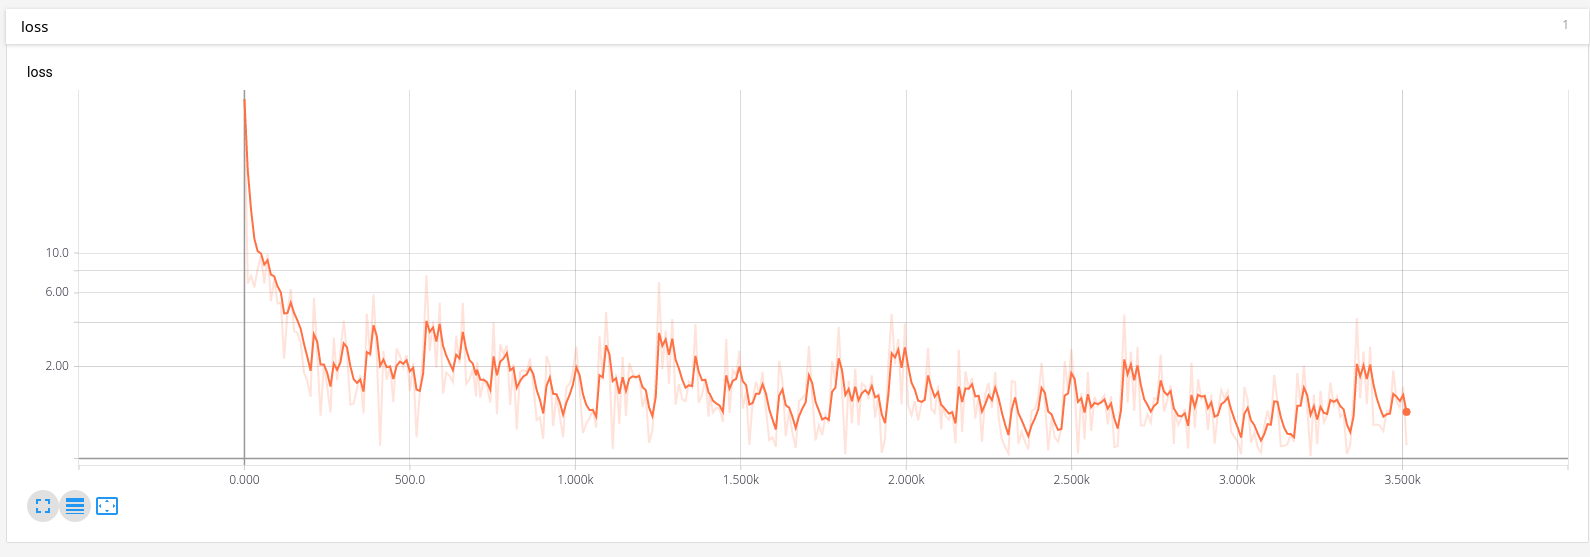
\includegraphics[width=6.5in]{images/loss.png}
  \caption {Loss diagram}
\end{figure}

Tensor board also provides a way of representing words. You can also see the links between Gloved words.

\begin{figure}[H]
  \centering
  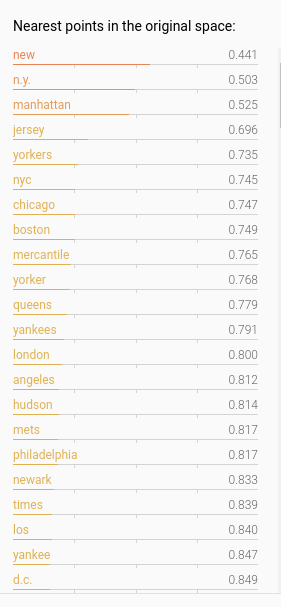
\includegraphics[width=2.5in]{images/york.png}
  \caption {Distance for word "York"}
\end{figure}
